\documentclass[12pt]{notes}

% Command for Questions
%\question{}

% Command for Notes
% \note{}

% Code to create a minipage where you can type in class notes. 
%%\begin{minipage}[l][2cm][c]{\textwidth}
%\begin{comment}

%\end{comment}
%%\end{minipage}

\usepackage{listings}

% In order for the minted code to run, we had to create a new compilation routine called pdflatex+shellEscape.
% This includes a --shell-escape command which should ONLY be used when pygmentized is required as it compromises security. 
% We also had to add pygmentize (a python package) to the system path (BEFORE miktex) and then restart the computer. 
\usepackage{minted}
\usemintedstyle{borland}
\lstset{language=SAS, 
  breaklines=true,  
  basicstyle=\ttfamily\bfseries,
  columns=fixed,
  keepspaces=true,
  identifierstyle=\color{blue}\ttfamily,
  keywordstyle=\color{cyan}\ttfamily,
  stringstyle=\color{purple}\ttfamily,
  commentstyle=\color{green}\ttfamily,
  } 
  
% \begin{minted}{sas}
% \end{minted}


% Begin Document
%==============================================================================
\begin{document}
% Include the Title of the Handout
\ntitle{4.3.1: Model Validation}

\begin{minted}{sas}
/* Project 2 is focused on using information regarding Tinder profiles 
to predict the genuineness of the user. Information regarding the total 
set of variables are included in the project 2 description. For purposes
of illustration, only a subset of variables are considered here. */

/* This first line of code will need to be changed */
FILENAME REFFILE '/home/u41171697/data/project2/tinder.csv';

PROC IMPORT DATAFILE=REFFILE replace
	DBMS=CSV
	OUT=WORK.tinder;
	GETNAMES=YES;
RUN;


/* Separate Into Training and Test Sets. 
Only Fit Models to the Training Set. The variable
"Selected" separates training (0) from test (1) 
seed - sets a random seed that allows your code to be reproduced
out - the name of the output dataset that includes the selected variable 
rate - the percentage of points (between 0 and 1) that will be "selected" 
       for validation */ 
proc surveyselect data=tinder seed=12345 out=tinder2
     rate=0.2; /* Withold 20% for validation */
run;

data train; set tinder2;
if Selected = 0;
run;

data test; set tinder2;
if Selected = 1;
run;

proc print data = train;
run;

/* Fit one model with 4 variables.  */
proc reg data=train noprint;
 model genuine = socprivconc instprivconc narcissism selfesteem;
store regModel;
run;

/* Fit another model with more variables.  */
proc reg data=train noprint;
 model genuine = socprivconc instprivconc narcissism selfesteem loneliness
                 hookup friends partner travel selfvalidation entertainment;
store regModel2;
run;

/* Fit a third model with NO variables  */
proc reg data=train noprint;
 model genuine = ;
store regModel3;
run;


/* Calculate MSPR for each model by first making predictions 
(via proc plm), then estimating errors (via a data step) and 
calculating the means (via proc means). */
proc plm restore=regModel;
 score data=test out=newTest predicted; 
 run;
 proc plm restore=regModel2;
 score data=test out=newTest2 predicted; 
 run;

proc plm restore=regModel3;
 score data=test out=newTest3 predicted; 
 run;


data newTest; set newTest;
ASE = (Genuine - Predicted)**2;
run;
data newTest2; set newTest2;
ASE = (Genuine - Predicted)**2;
run;
data newTest3; set newTest3;
ASE = (Genuine - Predicted)**2;
run;

proc means data = newTest;
var ASE;
run;
proc means data = newTest2;
var ASE;
run;
proc means data = newTest3;
var ASE;
run;
\end{minted}

\begin{figure}
\centering
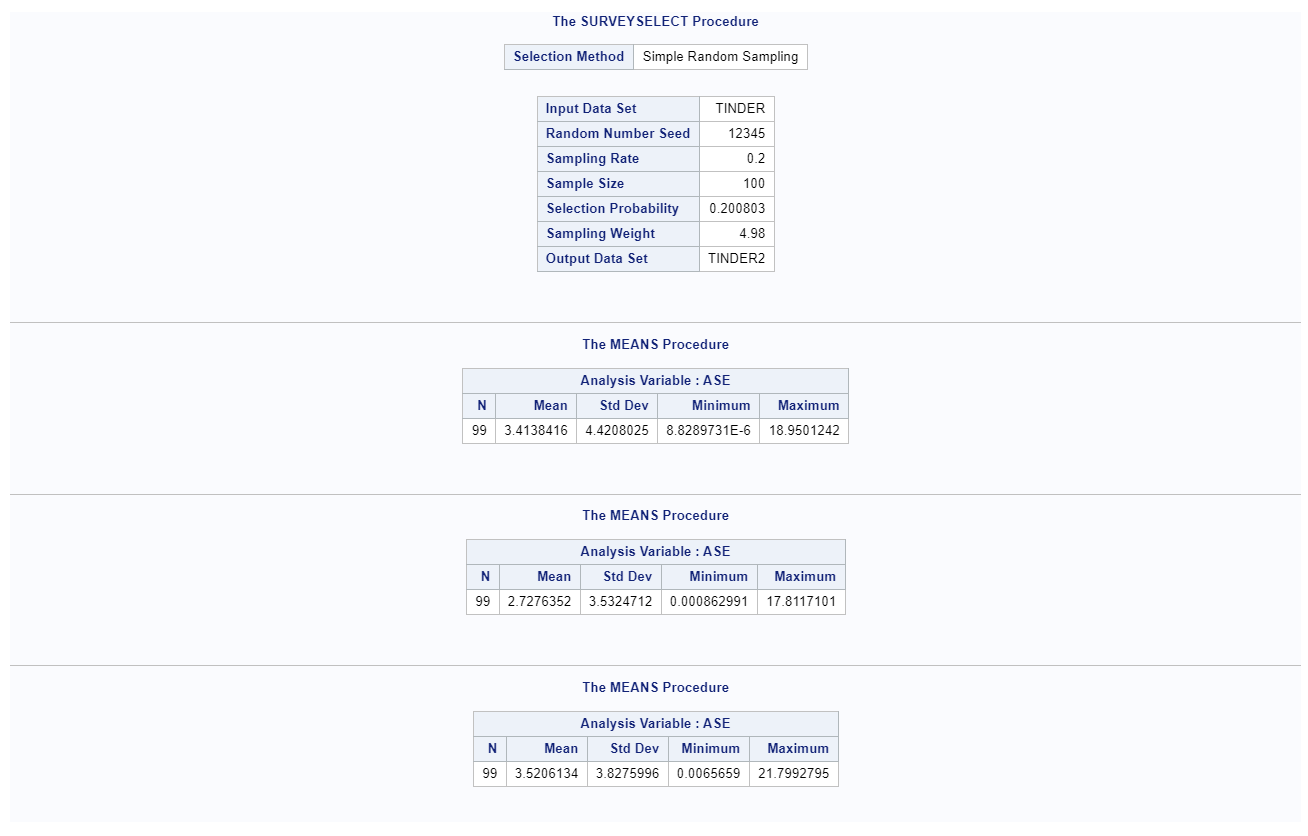
\includegraphics[width=\textwidth]{figures/module4/results_4_3_1.png}
\end{figure}











% End the Document
%==============================================================================
\end{document}